\documentclass[a4paper]{article}
\usepackage[utf8x]{inputenc}
\usepackage[T1,T2A]{fontenc}
\usepackage[russian]{babel}
\usepackage{hyperref}
\usepackage{indentfirst}
\usepackage{listings}
\usepackage{color}
\usepackage{here}
\usepackage{array}
\usepackage{multirow}
\usepackage{graphicx}
\usepackage{caption}
\graphicspath{{graphics/}}
\usepackage[left=2cm,right=2cm,
top=2cm,bottom=2cm,bindingoffset=0cm]{geometry}
\usepackage{listings}
\lstset{ %
	extendedchars=\true,
	keepspaces=true,
	language=bash,					% choose the language of the code
	basicstyle=\footnotesize,		% the size of the fonts that are used for the code
	numbers=left,					% where to put the line-numbers
	numberstyle=\footnotesize,		% the size of the fonts that are used for the line-numbers
	stepnumber=1,					% the step between two line-numbers. If it is 1 each line will be numbered
	numbersep=5pt,					% how far the line-numbers are from the code
	backgroundcolor=\color{white},	% choose the background color. You must add \usepackage{color}
	showspaces=false				% show spaces adding particular underscores
	showstringspaces=false,			% underline spaces within strings
	showtabs=false,					% show tabs within strings adding particular underscores
	frame=single,           		% adds a frame around the code
	tabsize=2,						% sets default tabsize to 2 spaces
	captionpos=b,					% sets the caption-position to bottom
	breaklines=true,				% sets automatic line breaking
	breakatwhitespace=false,		% sets if automatic breaks should only happen at whitespace
	escapeinside={\%*}{*)},			% if you want to add a comment within your code
	postbreak=\raisebox{0ex}[0ex][0ex]{\ensuremath{\color{red}\hookrightarrow\space}}
}

\begin{document}	% начало документа

\begin{titlepage}	% начало титульной страницы

	\begin{center}		% выравнивание по центру

		\large Санкт-Петербургский Политехнический Университет Петра Великого\\
		\large Институт компьютерных наук и технологий \\
		\large Кафедра компьютерных систем и программных технологий\\[6cm]
		% название института, затем отступ 6см
		
		\huge Телекоммуникационные технологии\\[0.5cm] % название работы, затем отступ 0,5см
		\large Отчет по лабораторной работе №3 \\[0.2cm]
		\large\textbf{"Линейная фильтрация"}\\[5cm]

	\end{center}


	\begin{flushright} % выравнивание по правому краю
		\begin{minipage}{0.25\textwidth} % врезка в половину ширины текста
			\begin{flushleft} % выровнять её содержимое по левому краю

				\large\textbf{Работу выполнила:}\\
				\large Власова А.В.\\
				\large {Группа:} 33501/4\\
				
				\large \textbf{Преподаватель:}\\
				\large Богач Н.В.\

			\end{flushleft}
		\end{minipage}
	\end{flushright}
	
	\vfill % заполнить всё доступное ниже пространство

	\begin{center}
	\large Санкт-Петербург\\
	\large \the\year % вывести дату
	\end{center} % закончить выравнивание по центру

\thispagestyle{empty} % не нумеровать страницу
\end{titlepage} % конец титульной страницы

\vfill % заполнить всё доступное ниже пространство

\section{Цель работы}
Изучить воздействие ФНЧ на тестовый сигнал с шумом.

\section{Постановка задачи}
Сгенерировать гармонический сигнал с шумом и синтезировать ФНЧ. Получить сигнал во временной и частотной областях до и после фильтрации. Сделать выводы о воздействии ФНЧ на спектр сигнала.


\section{Теоретический раздел}
Фильтр в обработке сигналов - устройство для выделения желательных компонентов спектра сигнала и/или подавления нежелательных. Фильтры бывают:
\begin{itemize}
	\item аналоговыми и цифровыми;
	\item пассивными и активными;
	\item линейными и нелинейными;
	\item рекурсивными и нерекурсивными.
\end{itemize} 

Линейный фильтр — фильтр, применяющий некий линейный оператор ко входному сигналу для выделения или подавления определённых частот сигнала и других функций по обработке входного сигнала. Линейные фильтры разделяются на два больших класса по виду импульсной переходной функции: фильтр с бесконечной импульсной характеристикой (БИХ-фильтры) и фильтр с конечной импульсной характеристикой (КИХ-фильтры). КИХ-фильтры могут быть осуществлены с помощью свёртки сигнала с импульсной характеристикой фильтра.\\

По тому, какие частоты фильтром пропускаются, фильтры подразделяются на:
\begin{itemize}
	\item фильтры нижних частот;
	\item фильтры верхних частот;
	\item полосно-пропускающие фильтры;
	\item полосно-задерживающие фильтры;
	\item фазовые фильтры.
\end{itemize}

Фильтр нижних частот (ФНЧ) - фильтр, эффективно пропускающий частотный спектр сигнала ниже некоторой частоты (частоты среза) и подавляющий частоты сигнала выше этой частоты. Степень подавления каждой частоты зависит от вида фильтра. В отличие от фильтра нижних частот, фильтр верхних частот пропускает частоты сигнала выше частоты среза, подавляя низкие частоты.


\section{Ход работы}
Сгенерируем гармонический сигнал, добавим к нему шум и выполним фильтрацию сигнала, используя фильтр Баттерворта.

\captionof{lstlisting}{}
\lstinputlisting{../lab3.m}

\begin{center}
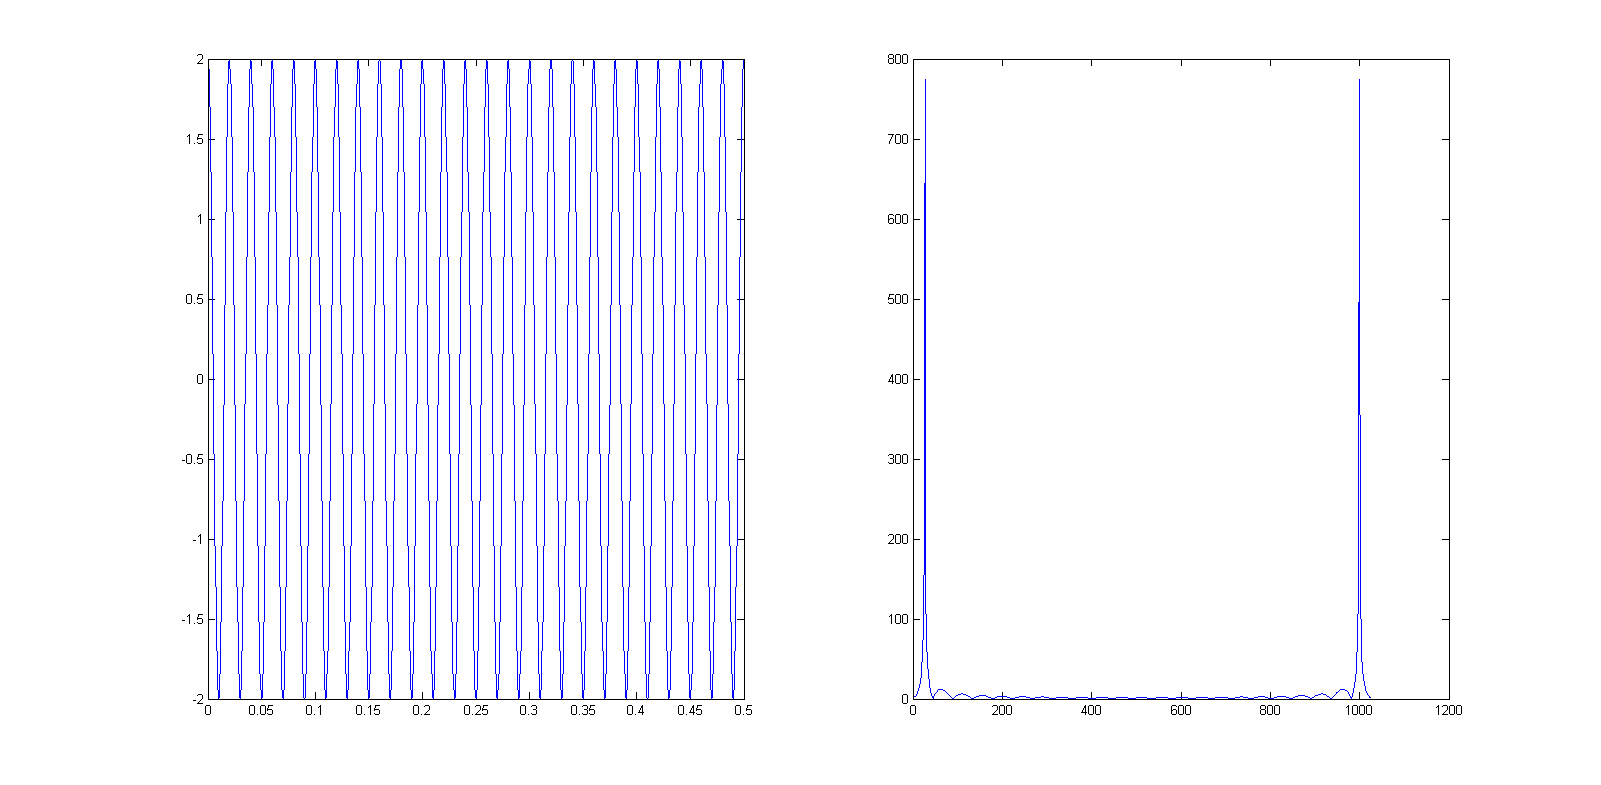
\includegraphics[scale = 0.4]{1.png}\\Рис.1 Сигнал до зашумления
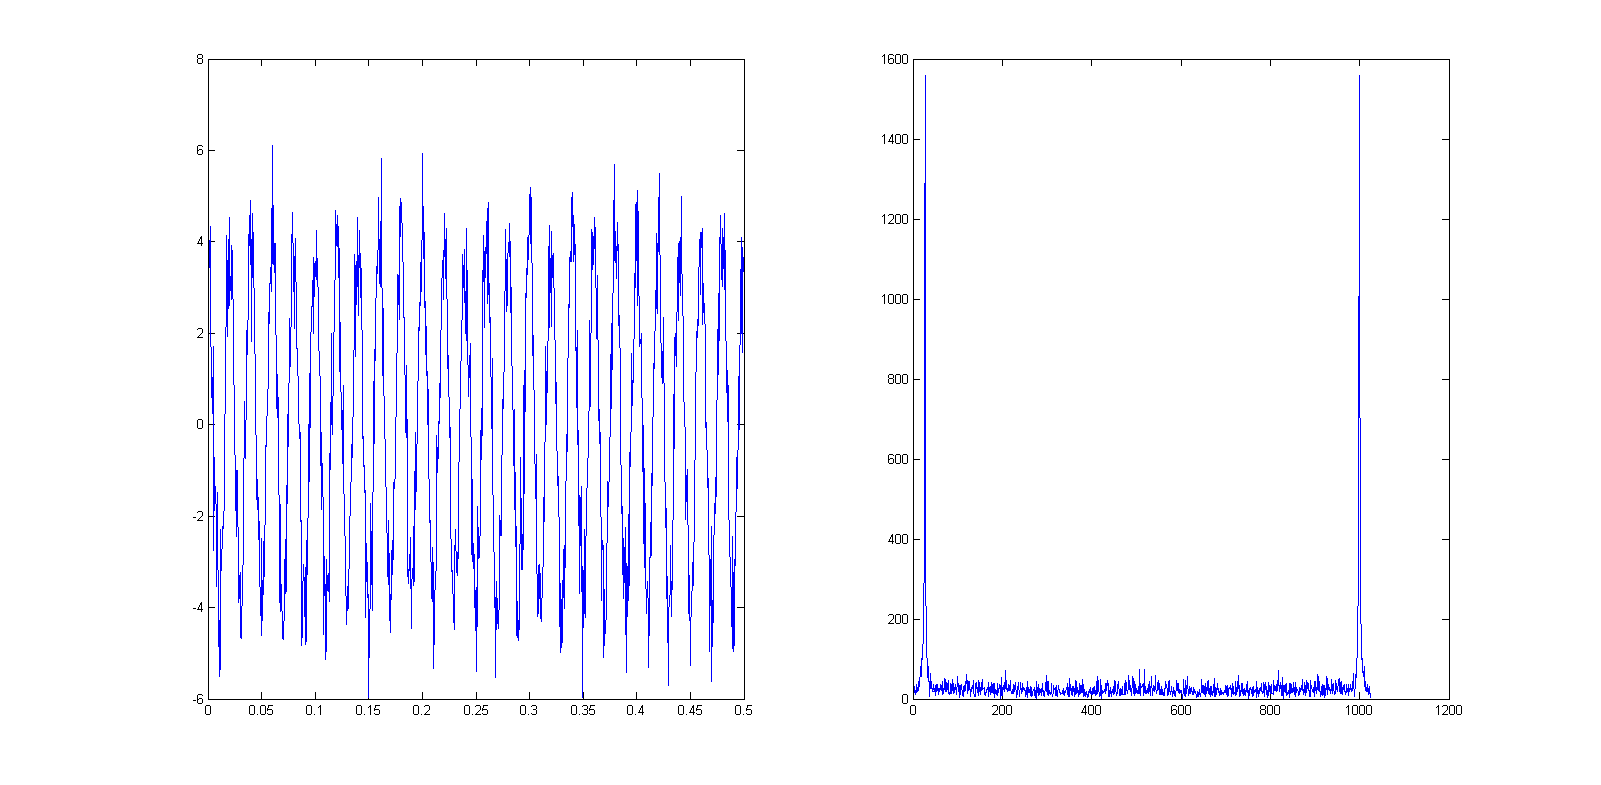
\includegraphics[scale = 0.4]{2.png}\\Рис.2 Сигнал после зашумления
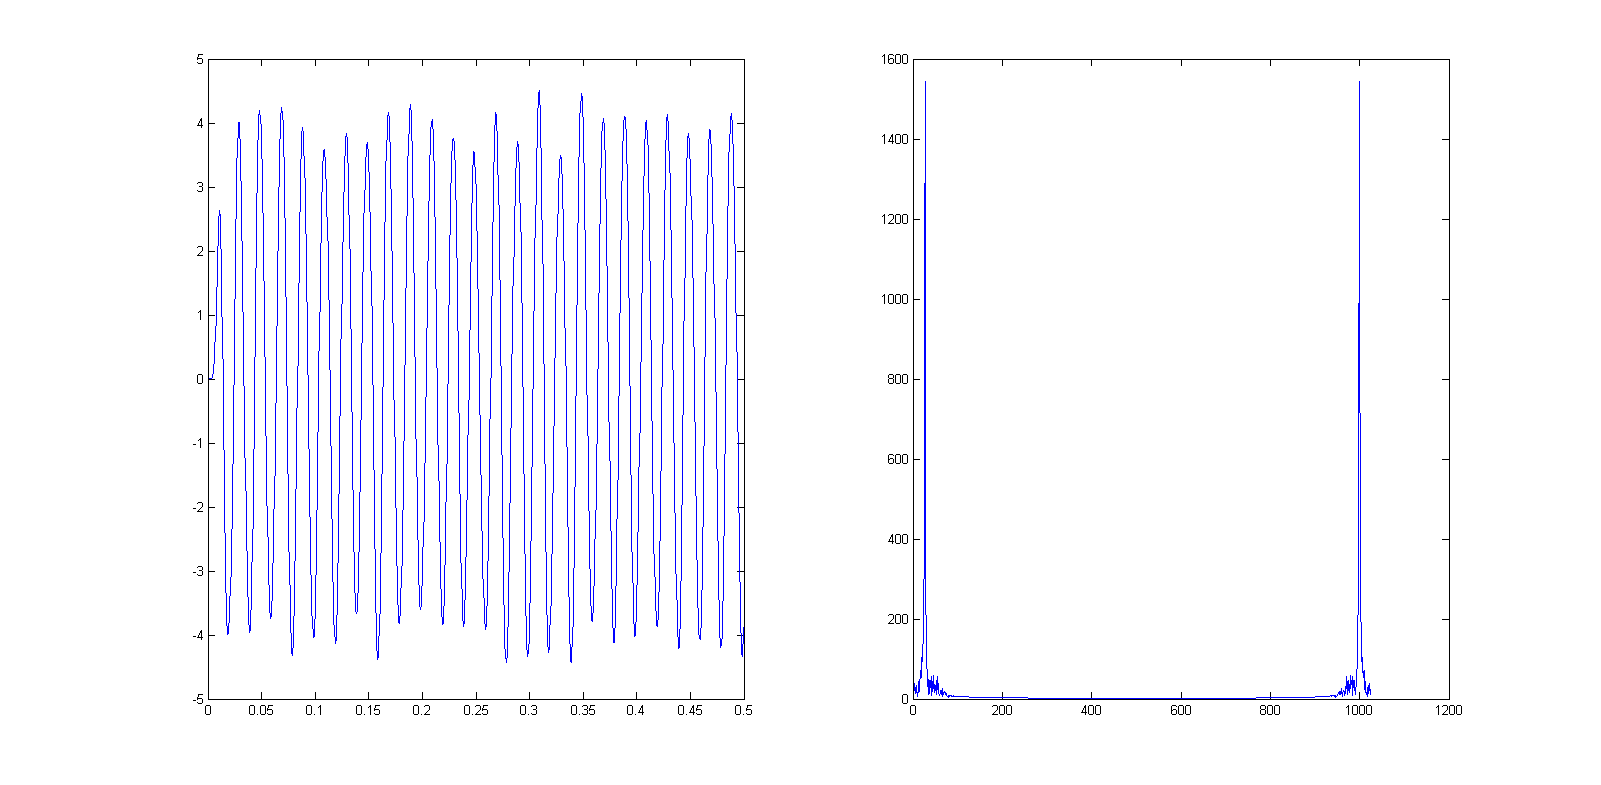
\includegraphics[scale = 0.4]{3.png}\\Рис.3 Сигнал после фильтрации
\end{center}

Проведем фильтрацию сигнала в среде Simulink.

\begin{center}
	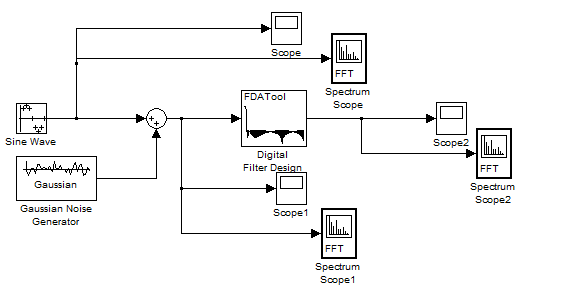
\includegraphics[scale = 1]{scheme.png}\\Рис.4 Схема в Simulink
\end{center}

На рис.5 представлен исходный сигнал, сигнал после зашумления и сигнал после фильтрации. На рис.6 - спектры сигналов соответственно.

\begin{center}
	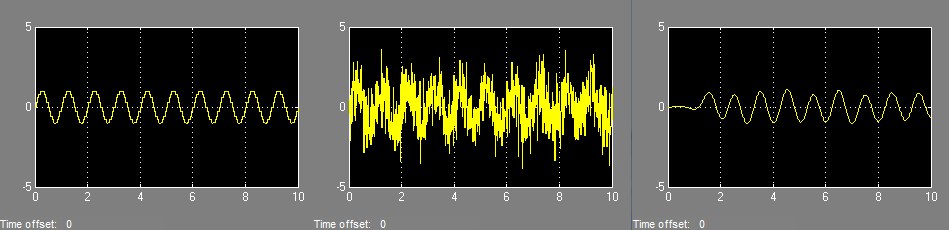
\includegraphics[scale = 0.7]{sim1.png}\\Рис.5 Сигналы в Simulink
	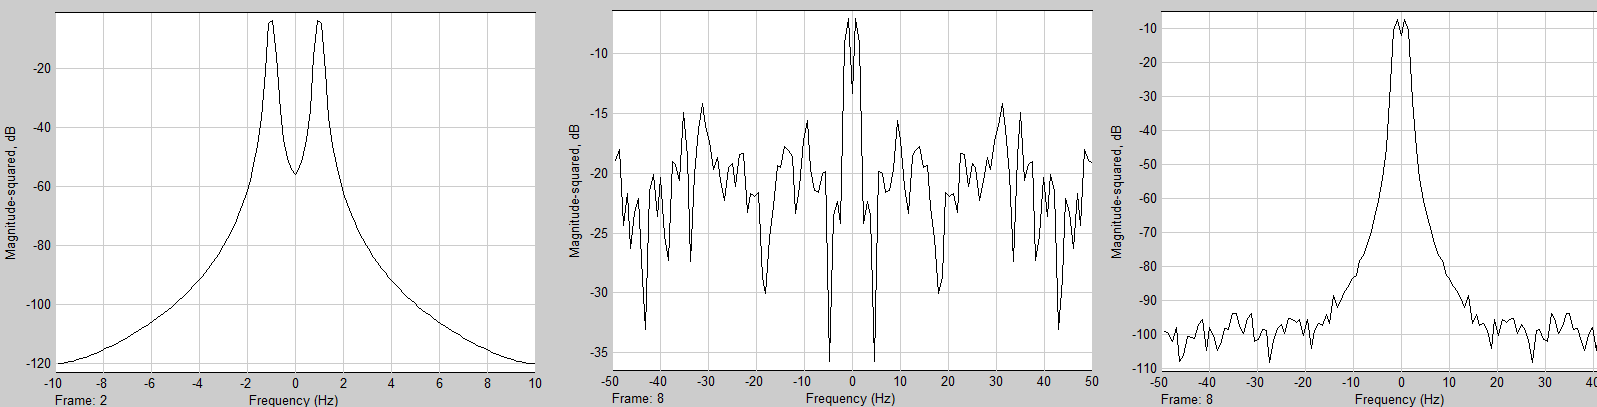
\includegraphics[scale = 0.4]{sim2.png}\\Рис.6 Спектры сигналов
\end{center}

\section{Выводы}
В ходе выполнения лабораторной работы исследован линейный ФНЧ и его воздействие на тестовый сигнал с шумом. По результатам видно, что сигнал после фильтрации не полностью совпадает с исходным. Это объясняется тем, что часть шума имеет низкие частоты, которые фильтр не может подавить.
\end{document}



